% 2011 年浙江卷文科第 18 题：f(x)=A sin(πx/3+φ) 的部分图象。
% 来源 PDF：普通高考/2011/2011浙江文.pdf，SHA-256 36931500dfd850579d93f0a685f0ccea25065c84c09db5157c451093d53b56f0。
% 原页：第 1 页第 3 栏，书页码 711。P(1,A) 最高点，Q(4,-A) 最低点，R(1,0)。
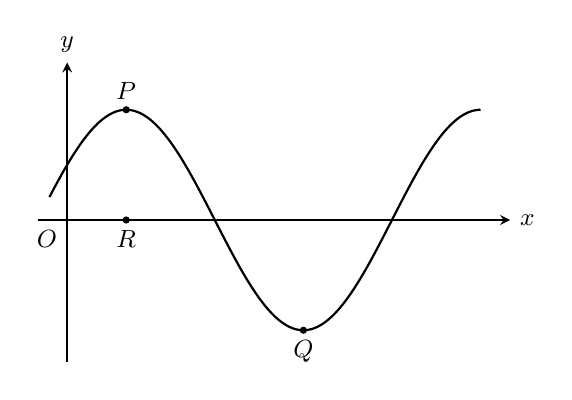
\begin{tikzpicture}[>=stealth, semithick, font=\small, x=0.75cm, y=1.0cm]
  \draw[->] (-0.5,0)--(7.5,0) node[right] {$x$};
  \draw[->] (0,-1.8)--(0,2.0) node[above] {$y$};
  \node[below left] at (0,0) {$O$};
  \draw[thick, domain=-0.3:7.0, samples=200] plot (\x,{1.4*sin(deg(pi*\x/3+pi/6))});
  \fill (1,1.4) circle (1.3pt) node[above] {$P$};
  \fill (4,-1.4) circle (1.3pt) node[below] {$Q$};
  \fill (1,0) circle (1.3pt) node[below] {$R$};
\end{tikzpicture}
